\documentclass[a4paper]{article}
\usepackage[utf8]{inputenc} % On explique à LaTeX que le fichier est de l'UTF8
\usepackage[french]{babel}  % On indique que le document doit suivre les conventions habituelles de la typographie française
\usepackage{graphicx,multirow} % Required for inserting images
\usepackage[table,xcdraw]{xcolor}
\usepackage{tabularx}
\usepackage{enumitem}
\usepackage{graphicx}
\usepackage{geometry}
\usepackage{float}
\usepackage{booktabs}
\usepackage{animate}
\usepackage{subcaption}
\usepackage{hyperref}
\date{\vspace{-3ex}}

\geometry{hmargin=2cm,vmargin=2cm}
\begin{document}
\title{Rapport de projet - Data Mining}
\author{Timothé BONHOURE - Jocelyn BOURNIER-ARMENI}
\maketitle
\tableofcontents
\vfill
À cause de la difficulté pour insérer des gifs dans un pdf, aucun gif n'a été inséré ici. Cependant dans le dossier \href{https://github.com/Jocelyn-Bournier/rplace_data_mining/tree/main/gif}{gif} de ce repo vous trouverez quelques gif qui avait été créer avant de se rendre compte de la difficulté.
\vfill
\begin{figure}[h]
    \centering
    \makebox[\textwidth][c]{\includegraphics[width=1.1\linewidth]{canvas.png}}
    \caption{Apercu du canvas}
    \label{fig:animated-gif}
\end{figure}

\newpage

\section{Introduction}

{L’objectif du projet était de réaliser une analyse sur un jeu de données réel, en utilisant les outils et techniques appropriés aux sujets que nous choisirions d'aborder. Le dataset que nous avons sélectionné est titré :`\textbf{Reddit 2023 r/place tile placement data}. L'événement r/place était une expérience sociale interactive qui a eu lieu sur la plateforme reddit, permettant aux utilisateurs du site de collaborer à la création d'\textbf{une grande grille de pixels}. Chaque utilisateur avait la possibilité de \textbf{placer un pixel toutes les cinq minutes sur la toile}, résultant en une œuvre collective en constante évolution. Le jeu de données que nous avons choisi d'explorer contient les informations relatives aux placements de pixel tout au long de l'événement. 
Une ligne du dataset contient pour un pixel posé, la date (au millième près), le nom d'utilisateur (hashé), l'emplacement et la couleur. 
Nous avons choisi, pour des raisons de performance, de nous concentrer sur un échantillon des données, toutes nos analyses seront ainsi réalisées en utilisant les deux premiers tiers des pixels placés.
Au cours de l'événement, la grille a été rallongée plusieurs fois, dans l'échantillon traité, elle a été étendue une fois de chaque côté, sur la verticale. Il a aussi été ajouté de nouvelles couleurs à la palette proposée.\\

Nous commencerons par une présentation des chiffres et statistiques générales sur le dataset. Ceci nous permettra de dimensionner les données et observer l'évolution de l'activité au cours du temps dans l'échantillon étudié. Ensuite, nous passerons à une partie concernant la recherche de différentes communautés qui ont pu se rassembler pour représenter des motifs particuliers sur la grille.\\

\section{Statistiques et présentation générale du dataset}

Sur l'échantillon traité, nous avons un total de presque 50 millions de pixels placés, dont 3 millions par les modérateurs pour retirer des motifs considérés comme inappropriés.

Une représentation graphique de la répartition spatiale de l'ensemble de l'activité sur le r/place est visible dans la figure \ref{fig:activite_total} ci-dessous. On y retrouve les zones de conflit auquel on pourrait s'attendre tel que la feuille d'érable du drapeau canadien. Mais aussi une zone un peu particulière qui est une zone dans laquelle a été réalisé une animation toute au long de r/place 2023 et qui a donc reçu une forte activité sans pour autant avoir fait l'objet de conflit. On remarque sur la figure \ref{fig:activite_total} que la zone centrale a une plus forte activité totale ce qui est normale, car cette partie était présente dès le début de r/place 2023 tandis que les deux parties sur les côtés ont été rajouté pendant l'événement.

\begin{figure}[h]
    \centering
    \includegraphics[width=.95\linewidth]{activite_total.png}
    \caption{Activité totale, de bleu (inactif) à rouge (très actif)}
    \label{fig:activite_total}
\end{figure}


Nous supposions et avons pu vérifier que le nombre de pixels placés par utilisateur, modélisant leur niveau d'investissement dans l'événement, devrait suivre une distribution en loi de puissance. Cette hypothèse s'est fortement confirmé après agrégation du nombre de pixels posés pour chaque utilisateur actif sur l'échantillon traité. La loi de distribution que nous avons obtenue est présentée dans la figure \ref{fig:pixel_placement_frequency_by_user}.

\begin{figure}[h]
    \centering
    \includegraphics[width=.50\linewidth]{pixel_placement_frequency_by_user.png}
    \caption{Fréquence de placement de pixels par utilisateur}
    \label{fig:pixel_placement_frequency_by_user}
\end{figure}

Nous avons aussi cherché à observer l'évolution de l'activité au cours de l'événement, tout en surveillant la répartition des différentes couleurs placées pour chacun des points, pour ce faire, nous avons réalisé plusieurs vues, la première, en figure \ref{fig:pixel_placement_frequency_by_color_global}, donne en chaque point un suivi du nombre de pixels posés sur les 5 dernières minutes, avec une moyenne lissé sur les 10 dernières minutes. Chaque aire sous la courbe d'une couleur représente le pourcentage de points placés de cette couleur à un instant t. On peut constater des creux qui se sont répétés sur les deux jours, représentant surement les horaires d'inactivités les plus probables pour les pays les plus impliqués, sachant que l'événement a démarrer à 13H UTC.

\begin{figure}[h]
    \centering
    \includegraphics[width=.80\linewidth]{pixel_placement_frequency_by_color_global.png}
    \caption{Moyenne glissante du nombre de pixels placés sur les 5 dernières minutes, par couleur}
    \label{fig:pixel_placement_frequency_by_color_global}
\end{figure}

\newpage 

La seconde (figure \ref{fig:pixel_placement_frequency_by_color_debut}), plus localisée sur le début de l'événement, permet de constater que les utilisateurs étaient plutôt synchronisés sur le placement des pixels au début, puis bien sûr une désynchronisation est vite survenue.

\begin{figure}[h]
    \captionsetup[subfigure]{justification=centering}
    \begin{subfigure}{.5\linewidth}
        \includegraphics[width=\linewidth]{pixel_placement_frequency_by_color_debut.png}
        \caption{Fréquence de placement par couleur \\ sur les premières heures de r/place 2023}
        \label{fig:pixel_placement_frequency_by_color_debut}
    \end{subfigure}
    \begin{subfigure}{.5\linewidth}
        \includegraphics[width=\linewidth]{pixel_placement_frequency_by_color_anomalie.png}
        \caption{Vue rapprochée de l'anomalie \\ de la fréquence de placement par couleur}
        \label{fig:pixel_placement_frequency_by_color_anomalie}
    \end{subfigure}
\end{figure}

Enfin, nous avons constaté en travaillant sur les données, une anomalie survenue au bout d'environ x heures, nous n'avons pas pu définir avec certitude la raison de cette anomalie, mais nous avons quelques hypothèses. Cette anomalie se présente par une chute dans l'activité des utilisateurs que l'on observe dans le zoom présenté en figure \ref{fig:pixel_placement_frequency_by_color_anomalie}. Durant l'événement, il y a eu plusieurs soucis de serveurs, mais non globaux en général, il est possible qu'un problème technique soit survenu pour tout le monde sur un intervalle de temps court. Ou il est possible que le souci vienne de l'enregistrement des données, peut-être que certains points placés ont été mal enregistrés.



\section{Recherche de communautés}
Nous avons cherché à détecter des communautés d'utilisateur. Pour cela nous nous sommes appuyé sur l’enchaînement sur chacun des pixels de différents utilisateur posant une couleur pour former un graphe. De ce graphe, nous déduisons alors les communautés grâce l'algorithme de Louvain.
\subsection{Approche l'ennemie de mon ennemie est mon amie}

\subsubsection{Idée de l'approche}

 Pour commencer, nous avons tout d'abord détecté des utilisateurs étant en opposition. Deux utilisateurs ayant placé l'un après l'autre sur le même pixel considéré en opposition. Nous avons fait ce choix, car lorsqu'un utilisateur mets un pixel juste après un autre, c'est qu'il souhaite changer la couleur que le précédent utilisateur avait mis. Nous avons de plus pondéré les liens entre les utilisateurs en fonction du nombre de fois que cela était arrivé 

Pour détecter des communautés à partir de ce graphe, nous avons utilisé une approche de type l'ennemie de mon ennemie est mon ami. Pour calculer le lien entre deux nœuds x,y nous avons regardé l'ensemble des ennemies commun aux deux nœuds, mais aussi si eux même étaient ennemies. Avec cela nous calculons un score de pondération des liens et on ne garde que les liens ayant un poids supérieur à un seuil. 

Une fois le graphe d'ennemie d'ennemie obtenu on réalise la détection de communauté vi l'algorithme de Louvain.

\subsubsection{Résultats}
Comme on peut le voir sur la figure \ref{fig:communities_sizes_ennemies} on obtient une très grande communauté avec un gros groupe de moyenne communauté (611 communautés ayant placé entre 3000 et 20000 pixels) et un énorme groupe de petite communauté (20000 communautés ayant placé moins de 100 pixels). 
\begin{figure}[h]
    \captionsetup[subfigure]{justification=centering}
    \begin{subfigure}{.55\linewidth}
        \includegraphics[width=\linewidth]{communities_sizes_ennemies.png}
        \caption{Distribution des tailles des communautés \\en échelle log-log}
        \label{fig:communities_sizes_ennemies}
    \end{subfigure}
    \begin{subfigure}{.4\linewidth}
        \includegraphics[width=\linewidth]{summary_enemies.png}
        \caption{Représentation des aires d'activité\\ des communautés\\ \tiny La couleur des pixels représente la communauté la plus active \\l'intensité du pixel à quel point la communauté a été active \\ par rapport aux autres communauté}
        \label{fig:summary_enemies}
    \end{subfigure}
\end{figure}

On remarque sur la figure \ref{fig:summary_enemies} que les communautés sont assez mal séparé. En effet seuls certaines ressorte en un emplacement du canvas et les autres donne plus l'impression d'un bruit.

\subsubsection{Limites de l'approche}
Cette approche possède plusieurs défaut qui explique pourquoi nous n'avons pas réussis à detecter de belle communauté : 
\begin{description}
    \item[Lenteur de calcul :] Comme on doit parcourir l'ensemble des ennemis de chacun des ennemis de chacun des nœuds cela représente énormément de lien possible ce qui est extrêmement lent.
    \item[Difficulté de choisir un seuil :] En effet le facteur seuil à un rôle crucial, car il va influencer la densité du graphe et par voie de conséquence impacter la taille et forme des communautés. Si on coupe trop haut on risque de perdre des informations importantes pour la détection des communautés. Si on coupe trop bas l'algorithme prendra trop de temps à cause du nombre important de lien. De plus le score qui a été calculé pour indiquer à quel point deux nœuds partage des ennemies en commun a été choisi arbitrairement et d'autre manière de le calculé pourrait donner de meilleurs résultats.
    \item[Problème du multi-communautarisme :] En effet, si deux communautés sont en conflit alors utilisé les conflits entre les utilisateurs pour trouver des voisins dans les ennemis des ennemis fonctionne bien. Mais le problème, c'est que chaque utilisateur n'appartient pas qu'à une seule communauté. Ainsi, il peut avoir un ennemi au titre d'une communauté et un autre au titre d'une autre communauté. Et alors les deux ennemis n'ont aucune raison d'avoir un lien particulier. Or avec l'approche ici développé ils peuvent en avoir à partir du moment ou les deux communautés ont une intersection suffisamment grande.
    \item[problème de l'animation :] Comme discuté plus tôt parmi toutes les œuvres l'une d'entre elles resort grâce à sa particularité elle n'est pas statique, mais évolue tout au long de l'événement et vise à reproduire l'animation \href{https://www.reddit.com/r/place/comments/15bvtcu/bad_apple_rplace_2023_and_original_side_by_side/}{Bad Apple} Cette communauté va en permanence remplacer ces propres pixels ce qui risque de trop réduire leur score qui prend en compte en plus de leurs ennemis en commun le fait qu'ils soient ou non ennemis.
\end{description}


\subsection{L'approche celui qui combat mon ennemi est mon amie}

\subsubsection{Idée de l'approche}
L'Idée de cette version améliorée de l'approche précédente est d'au lieu de considéré tous les ennemis de mes ennemis, je peux considérer uniquement ces ennemis qui m'aident à le combattre. Pour cela on va considérer comme amis deux utilisateurs tel que l'un d'entre eux a remis le même pixel que l'autre juste après qu'il ait été changé.
Le premier avantage est que cela est bien plus facile à calculer, en effet il suffit d'itérer sur l'ensemble du dataset et chaque action ne pourra donner qu'une seule liaison dans le graphe. Cela nous permet de lancer cette approche sur l'ensemble du dataset à disposition. Le deuxième gros avantage est que le choix sur les ennemis de nos ennemis étant fait sur le même pixel on s'assure d'avoir une certaine localité à notre communauté.

Malgré que cela soit bien plus rapide et que nous puissions le faire tourner sur l'ensemble des 50 heures que nous nous étions fixé comme échantillon l'ensemble des traitements à tout de même pris plus de deux heures. En particulier l'algorithme de Louvain à lui seul à pris plus d'une heure.

\subsubsection{Résultats}
Comme on peut le voir sur la figure \ref{fig:communities_sizes_friends} on obtient cinq très grande communauté (plus de quatre millions de pixels placé) suivi d'une trainée de grosse communauté (17 communauté ayant placé entre 100K et 2M) ce finissant par un gros groupe de moyenne communauté (77 communautés ayant placé entre 10000 et 100000 pixels) et un énorme groupe de petite communauté (10816 communautés ayant placé moins de 2000 pixels). 
\begin{figure}[h]
    \captionsetup[subfigure]{justification=centering}
    \begin{subfigure}{.45\linewidth}
        \includegraphics[width=\linewidth]{communities_sizes_friends.png}
        \caption{Distribution des tailles des communautés \\en échelle log-log}
        \label{fig:communities_sizes_friends}
    \end{subfigure}
    \begin{subfigure}{.55\linewidth}
        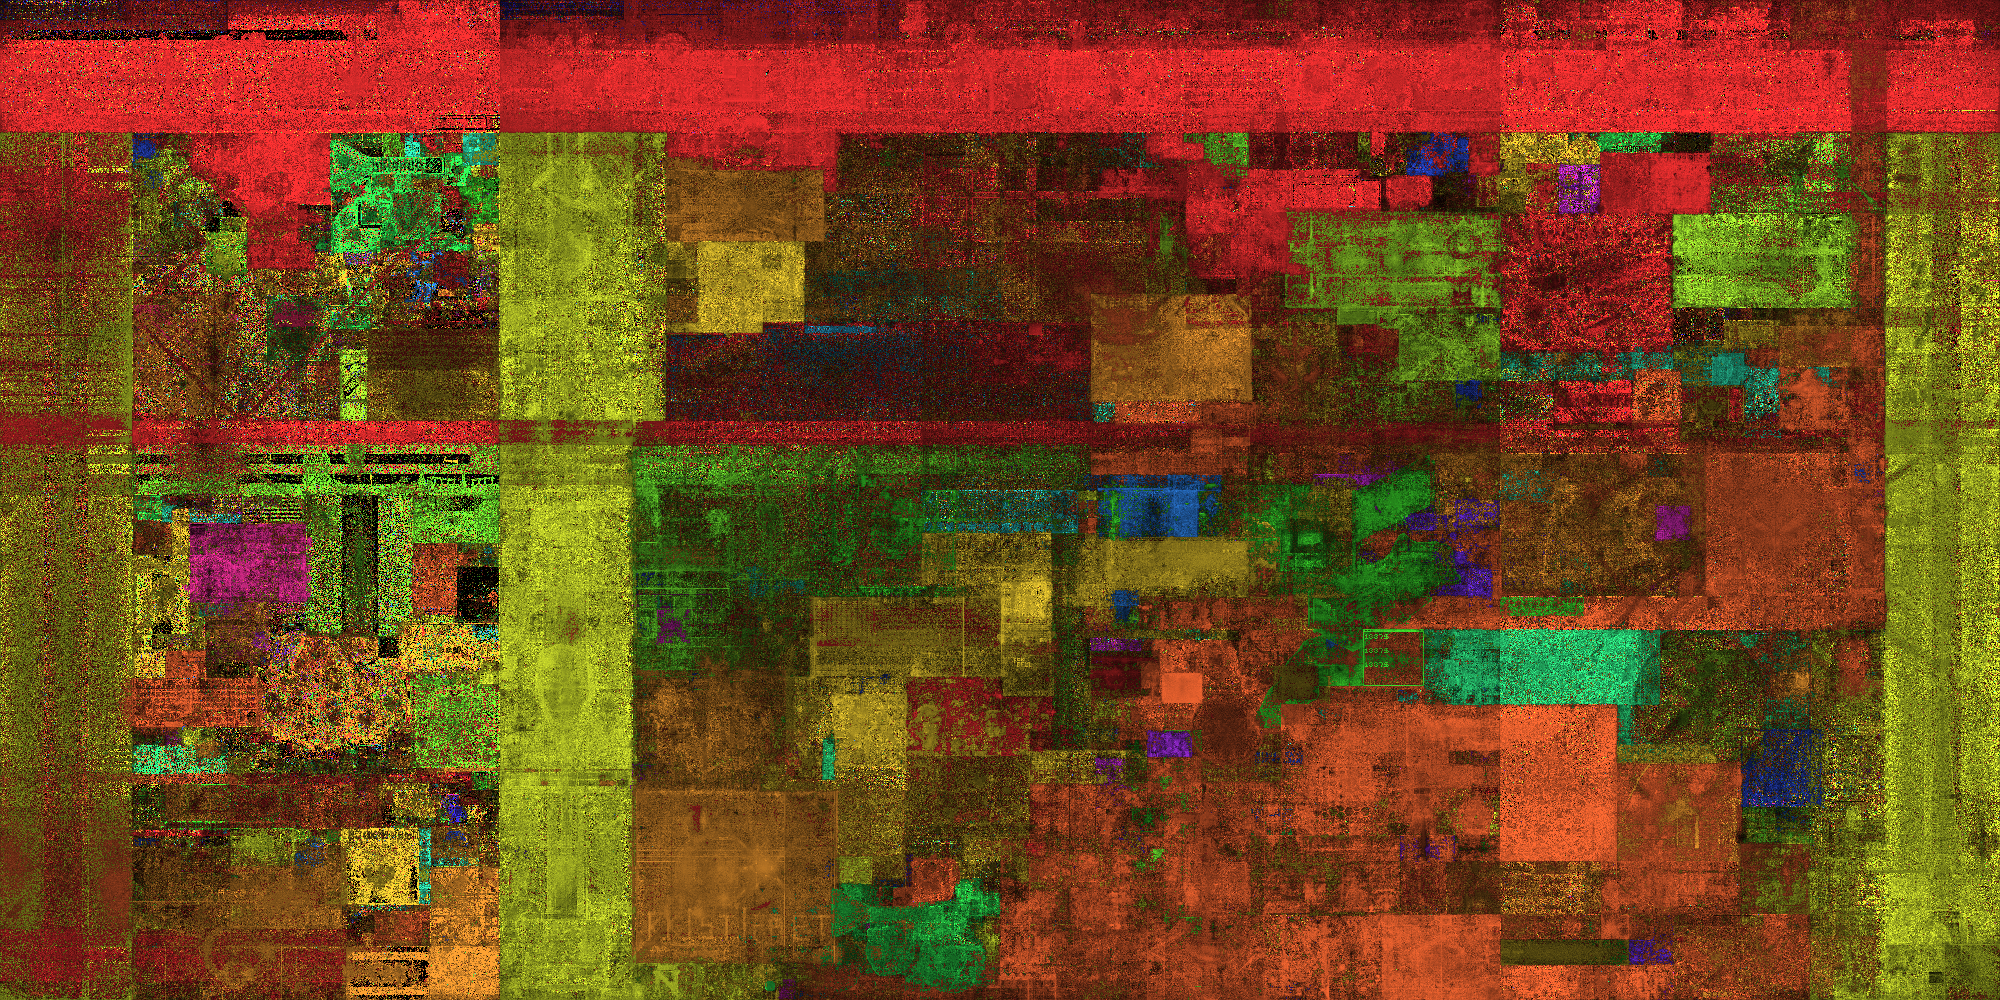
\includegraphics[width=\linewidth]{summary_friends.png}
        \caption{Représentation des aires d'activité\\ des communautés\\ \tiny La couleur des pixels représente la communauté la plus active \\l'intensité du pixel à quel point la communauté a été active \\ par rapport aux autres communauté}
        \label{fig:summary_friends}
    \end{subfigure}
\end{figure}

On remarque sur la figure \ref{fig:summary_enemies} que les communautés sont bien séparé et peuvent être facilement associé à de véritable communauté. Ainsi on peut remarquer que le rouge correspond à la communauté allemande tandis que le jaune correspond à la communauté française. En regardant d'autre communauté parmi les plus actives on remarque facilement qu'elle corresponde à une ou plusieurs œuvres d'art. De plus on peut même voir des zones de luttes entre deux communautés par exemple sur l'extrême gauche du canvas on voit un mélange des couleurs jaune et rouge. En regardant l'évolution du canvas on remarque que cette zone correspondait à un drapeau français avant qu'il ne se fasse détruire à la toute fin de notre échantillon, c'est donc cela que l'on voit.
\subsubsection{Limites de l'approche}      
Malgré que cette approche fournisse de belle communauté on peut remarquer qu'elle a toujours tendance à rassembler ensemble des communautés qui ne semble pas en former qu'une seule. Par exemple
la communauté technoblade est inclus dans la communauté allemande, cependant technoblade semble être une chaîne YouTube de jeux vidéo en anglais. Il n'y a pas de raison que ce soit la même que les Allemands. Une possibilité est simplement que ces communautés ont une intersection suffisamment grande pour que l'algorithme les fusionne plutôt que de séparé entre deux communautés ceux qui appartiennent aux deux. On voit donc bien ici la limite du fait de supposer que chaque utilisateur appartient à une unique communauté.
\section{Conclusion}
Ainsi nous avons pu étudier des statistiques générales du dataset. Nous avons réalisé une étude succincte de la fréquence de placement par couleur. Et finalement, nous avons réalisé une recherche de communauté qui s'est avéré fructueuse. 
Si nous avions eu plus de temps, nous aurions aimé croiser les aspects de fréquence de placement et de recherche de communauté. Des questions que nous aurions aimées nous poser sont : 
\begin{enumerate}
    \item Comment les profils de fréquence varie en fonction de la communauté ?
    \item Est-on capable de différencier des communautés qui serait plutôt territorial (français, allemand, espagnol) de communauté plus répandue uniformément~?
    \item Est-on capable de retrouvé des communautés à partir uniquement des fréquences de placement de pixel~?
    \item Est-on capable d'améliorer les prédictions de communauté déjà réalisée~? En particulier est-on capable de séparer les communautés qui ont été fusionné à tort.
\end{enumerate} 
\end{document}